\chapter{Marco teórico}
\label{Marco_teorico}

%\section{Estudio de mercado}
%A lo largo de los años los \ac{RTS} siempre han contado con una gran aceptación entre
%los usuarios de \ac{PC}, un claro ejemplo de esto puede ser el juego \textit{`Age of
%Empire II: The Age of Kings'}\footnote{Desarrollado por `Ensemble Studios' y lanzado a
%finales de 1999.} el cual se posicionó como uno de los juegos más vendidos del momento
%superando el millón de copias. Actualmente el juego cuenta con una remasterización
%\footnote{Co-desarrollado por Forgotten Empires, Tantalus Media y Wicked
%Witch. Lanzado en noviembre de 2019.} la cual ha conseguido vender más de 50.000
%copias en \textit{`Steam'}. Datos extraídos de su articulo en \citeauthor*{Wiki_AoE2}.

%Si miramos en el panoráma nacional actual, podemos encontar el juego \textit{`They Are
%Billions'} \footnote{Desarollado por Numantian Games y lanzado en junio de 2019.}
%disponible inicialmente para \ac{PC} y posteriormente lanzado en \textit{`PlayStation 4'}
%y \textit{`Xbox One'} debido a su éxito. A día de hoy el juego a conseguido vender
%solamente en \textit{`Steam'} más de 25.000 unidades consiguiendo una valoración muy
%positiva por parte de los usuarios de la plaforma como podemos ver en la página 
%del juego de \citeauthor*{TaB2019} en dicha tienda.

%El género puede aparentar ser cosa del pasado pero vistas las cifras podemos concluir
%que sigue siendo un reclamo para los jugadores.

\section{Referentes}
Cuando uno busca desarrollar un producto es una buena práctica el investigar que se ha realizado
previamente en entregas similares, ver que ténicas se han utilizado y que problemas se han
encontrado y como los solventaron. También es interesante ver que mecánicas se han ido consevando
y que innovaciones se han ido introduciendo con el paso del tiempo.

A continuación vamos a detallar aspectos de interés encontrados en diversas entregas
las cuales nos servirán de referentes.

\subsection{Age of Empires II: The Age of Kings}
En primer lugar encontramos el juego \textit{'Age of Empires II: The Age of Kings'}, en
este juego encontraremos una serie de campañas a través de las cuales encarnaremos a personajes
históricos como `Juana de Arco' o `William Wallace' y los acompañaremos en sus conquistas y
batallas más icónicas. Además de grandes batallas encontraremos el deber de gestionar nuestra
facción, este trabajo nos requerirá recoger rescursos a lo largo del mapa mientras desarrollamos 
nuestras ciudades y unidades.

El desarrollo tecnológico se divide en cuatro etapas históricas: Alta Edad Media,
de los castillos, Feudal e Imperial. Cada una de estas etapas trae consigo una serie de
unidades, edificaciones e investigaciones nuevas las cuales nos proporcionaran escenarios
más complejos a nivel estratégico, para pasar de una etapa a otra no es necesario completar
al 100\% las opciones desbloqueadas, solo unos requisitos mínimos.

El juego cuenta con un total de 35 civilizaciones o facciones, todas tienen acceso al mismo árbol
tecnológico pero cuentan con ligeras diferencias, cada una cuenta con una o dos tecnologías únicas
y características especiales en una unidad militar\footnote{Normalmente alguna cualidad mejorada en relación a las
demás como puede ser la velocidad o daño.}.

Todas la unidades militares\footnote{Lista de unidades: \url{https://ageofempires.fandom.com/wiki/Units_(Age_of_Empires_II)}.}
de las que podemos disponer cuentan con una serie características que
las hacen más o menos fuertes en función del objetivo al que se enfrenten, podemos encontrar
el ejemplo de las máquinas de asedio las cuales son más fuertes contra estructuras pero
más débiles contra infanteria, o las unidades a caballo que son fuertes contra arqueros
e infanteria pero débiles frente a lanceros. \\
Este tipo de mécanicas dotan al juego de una importante componente táctica en el manejo
de las unidades que debemos dominar si queremos completar los diferentes niveles de
forma satisfactoria~\ref{img:aoe_2}.

\begin{figure}[ht]
\centering
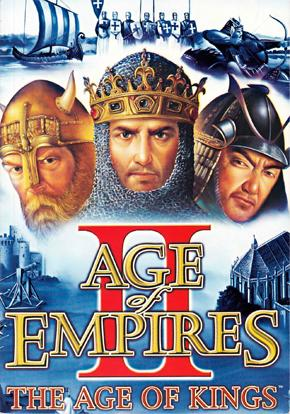
\includegraphics[width=0.3\textwidth]{imagenes/marco_teo/referentes/aoe_1.png}
\caption{Carátula del juego original.}
\label{img:aoe_1}
\end{figure}

En lo referente a edificaciones\footnote{Lista de edificios: \url{https://ageofempires.fandom.com/wiki/Buildings_(Age_of_Empires_II)}.}
podemos encontrar distintos tipos según su aporte al jugador,
el edifício printipal es el `Ayuntamiento' el cual nos permitirá crear colonos para que trabajen
recogiendo recursos y/o ayudando en la construcción de nuevas estructuras, en segundo lugar podemos
encontrar edifícios como el `Cuartel' o el `Campo de tiro' los cuales nos permiten crear unidades
militares, por otro lado tenemos edificios como la `Herreria' la cual nos permitirá realizar investigaciones
y crear unidades de asedio.

Por último podemos encontrar estructuras de temática religiosa como el `Monasterio', otras destinadas
a aumentar la productividad en las explotación de recursos naturales como el `Molino'
y defensivas como las `Murallas'. 

\begin{figure}[ht]
\centering
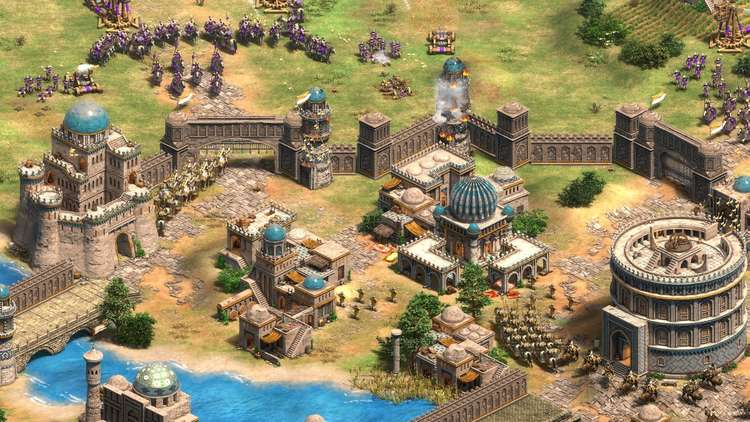
\includegraphics[width=0.7\textwidth]{imagenes/marco_teo/referentes/aoe_2.png}
\caption{Ciudad siendo asediada.}
\label{img:aoe_2}
\end{figure}

En el género \ac{RTS} hay una tendencia al uso de una perspectiva isométrica con cámara fija
la cual solo podemos modificar haciendo zoom o desplazandola por el entorno, esto seguramente
se deba a que es la configuración que mejor nos permite observar el mapa y todas las unidades que
hay en el. Además, el hecho de que sea fija nos libra de la problemática de ir ajustando la
cámara según la parte del mapeado que estemos observando, ya que, seguramente el mapeado y los elementos
visuales del juego también hayan sido diseñados teniendo esto en cuenta.

Como podemos ver en el artículo de \citeauthor*{Pritchard2000} sobre el desarrollo de \ac{AoE} 2,
la \ac{IA} del juego esta desarrollada completamente con un lenguaje de \textit{scripting} desarrollado
por ellos~\ref{img:aoe_scripting_1}, de esta forma el código consiste en una serie de constantes y variables definidas desde un
inicio y mediante condicionales realizar las acciones  y cambios pertinentes. Gracias a un usuario
de \textit{`GitHub'} podemos ver en las imagenes~\ref{img:aoe_scripting_2} el código usado en el juego, la extensión es 
de  más de 10.000 líneas de código.

\begin{figure}[ht]
\centering
\begin{minipage}[c]{0.45\linewidth}
	\hspace{9mm}
	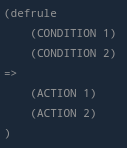
\includegraphics[height=0.15\textheight]{imagenes/marco_teo/referentes/aoe_scripting_1.png}
	\caption{Descripción Estructura.}
	\label{img:aoe_script_1}
\end{minipage}
\begin{minipage}[c]{0.45\linewidth}
	\hspace{9mm}
	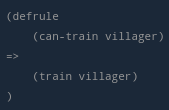
\includegraphics[height=0.15\textheight]{imagenes/marco_teo/referentes/aoe_scripting_2.png}
	\caption{Ejemplo condición.}
	\label{img:aoe_script_2}
\end{minipage}
\textbf{Fuente:} guía de scripting para \ac{IA} de \ac{AoE} 2 de \citeauthor*{redmechanic2017}.
\label{img:aoe_scripting_1}	
\end{figure}

\begin{figure}[ht]
\centering
\begin{minipage}[c]{0.45\linewidth}
	\hspace{9mm}
	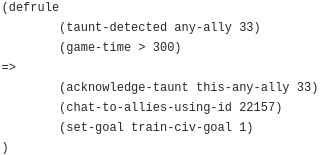
\includegraphics[height=0.11\textheight]{imagenes/marco_teo/referentes/aoe_scripting_3.png}
	\caption{Ejemplo condición.}
	\label{img:aoe_script_3}
\end{minipage}
\begin{minipage}[c]{0.45\linewidth}
	\hspace{9mm}
	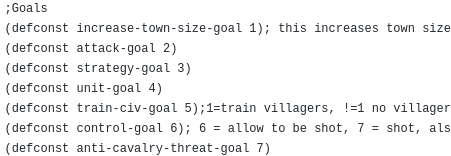
\includegraphics[height=0.11\textheight]{imagenes/marco_teo/referentes/aoe_scripting_4.png}
	\caption{Ejemplo constantes.}
	\label{img:aoe_script_4}
\end{minipage}
\textbf{Fuente:} repositorio de \textit{'GitHub'} del usuario \citeauthor*{Andygmb2014}. 
\label{img:aoe_scripting_2}	
\end{figure}

Además de estos \textit{scripts} el juego utiliza un sistema de \textit{pathfinding} en dos niveles,
el primero de los algoritmos calcula la ruta a seguir por las unidades sin tener el cuenta los
elementos triviales como las demás unidades, mientras que la segunda pasada calcula el camino 
en tramos específicos con el fin de esquivar otras unidades, edificaciones, etc...

En lo referente al movimiento de las unidades, tanto por la forma en la que está programada
la \ac{IA} como por la sensación que dan al jugar, es posible que se trate de un  \textit{``Goto''}
clásico y sencillo para evitar realizar muchos cálculos. \\
Además, con el tiempo el juego se ha convertido en un objetivo para \textit{``Speedrunners''}
y con una escena competitiva que se basa en ser el más rápido jugando\footnote{En los enfrentamientos de alto rango se llegan a medir las acciónes por minuto (APM).}
por lo que una reacción instantánea de las unidades es un factor importante para  estos
jugadores.

\subsection{The Are Billions}
En segundo lugar podemos encontrar el +juego \textit{'\acf{TaB}'} el cual reutiliza
una serie de características propias del género y como pueden ser la perspectiva
isométrica pero sin dejar de innovar introduciendo nuevas mecánicas y/o formas de
plantear la jugabilidad.

\begin{figure}[ht]
\centering

\includegraphics[width=0.7\textwidth]{imagenes/marco_teo/referentes/tab_1.png}
\caption{Imágen promocional del juego.}
\label{img:tab_1}
\end{figure}
 
En \textit{'\ac{TaB}'} podemos encontrar funciones interesantes como la pausa
táctica la cual nos permitirá visualizar detenidamente el estado del mapa sin tener que
preocuparnos por no estar atendiendo algunos posibles eventos como ataques a nuestras
tropas por parte del enemigo. En juegos anteriores como los \textit{'\ac{AoE}'} es
fácil encontrarnos en la situación de tener trabajadores en la ciudad sin hacer tareas
un rato y no poder mirar cuales son e ir pensando su ocupación siguiente por estar
atrapado en refriegas con otros jugadores, con este tipo de mecánicas estas situaciones
se solventan en mayor o menor medida y permiten al jugador tomarse el tiempo que
necesite para pensar las acciones que quiere realizar.

Otro aspecto llamativo en el podemos fijarnos es en la aparición de solamente dos
facciones. Por un lado encontramos `El Nuevo Imperio', la facción del jugador, la
cual representa una serie de colonias que tendremos que desarrollar a lo largo de
los niveles. En el otro lado encontramos las infinitas hordas de zombis que tratarán
de exterminar a la raza humana.

\begin{figure}[ht]
\centering
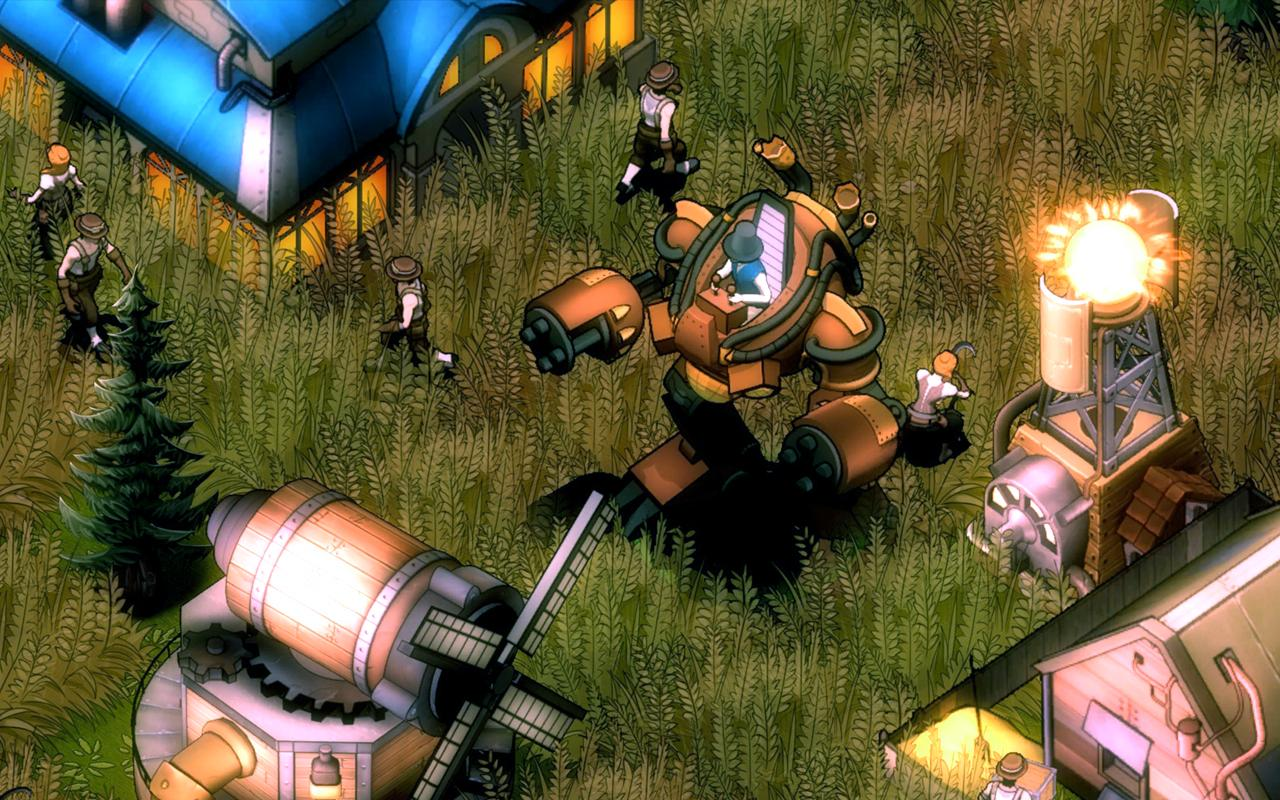
\includegraphics[width=0.6\textwidth]{imagenes/marco_teo/referentes/tab_2.png}
\caption{Ejemplo de unidad mecánica del imperio y estética del juego}
\label{img:tab_2}
\end{figure}

A diferencia de en \textit{'\ac{AoE}'} que todas la facciones poseen las mismas unidades
\footnote{Algunos valores pueden variar según bonos de facción}, en
\textit{'\ac{TaB}'} cada facción dispondrá de unidades únicas con acciones propias.
Como podemos ver en la imágen~\ref{img:tab_2} las tropas del imperio se basan en el uso
de maquinaria y armas de fuego para repeler las hordas enemigas, por otro lado los
zombis contarán con diversas caraterísticas físicas mejoradas conforme sean de mayor
``nivel'' puediendo encontrar algunos más rápidos, o más fuertes o más grandes y
resistentes al daño.~\ref{img:tab_3}

\begin{figure}[ht]
\centering
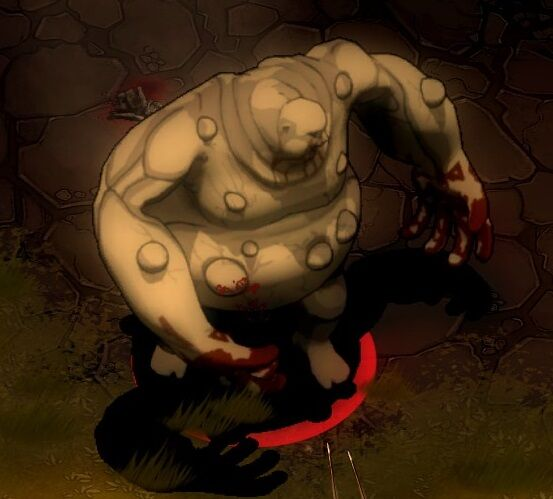
\includegraphics[width=0.5\textwidth]{imagenes/marco_teo/referentes/tab_3.png}
\caption{Infectado gigante}
\label{img:tab_3}
\end{figure}

Como último punto a destacar de la entrega tenemos la introducción del un modo de
juego de supervivencia donde a lo largo del tiempo irán apareciendo oleadas de zombis
donde cada vez aparecen más enemigos y más poderosos de forma infinita, haciendo así
que la partida termine cuando el jugador deje de aguantar la ofensiva enemiga.


\section{Técnicas de inteligencia articificial}
Como ya se ha mencionado anteriormente en la introducción~\ref{intro} de este \ac{TFG}
el grueso del desarrollo y uno de los objetivos más importantes del proyecto recaen en
el desarrollo de una \ac{IA} haciendo uso de las técnicas de \textit{'Flocking'} y
\textit{`Steering behaviors'}.

Para ello nos basaremos principalmente en las explicaciones y ejemplos que podemos
encontrar en el libro \cite[ch.~3]{Millington2009} donde de forma extensa y detallada
se nos introduce en la teoría relacionada a los algoritmos y la forma en la que estos
se estructuran e interactuan entre ellos. Para dar un poco de contexto sobre el tema
resumiremos brevemente las ideas que se nos presentan a lo largo del capitulo dedicado
a estas técnicas. 

Los \textit{`Steering behaviors'} pueden ser entendidos como una serie de algoritmos
destinados a guiar la forma en la cual los \ac{NPC} se desplazan por el escenario
y/o interactuan con los distintos elementos que puedan encontrase en la escena. Siguen
una filosofía de crear movimientos complejos a base de una combinación de movimientos 
y/o acciones simples, un ejemplo común puede ser la acción de perseguir a un objetivo
mientras se sortean obstáculos en el proceso. \\ 
En este caso no tendríamos una función llamada 
\textit{``persigue-enemigo-mientras-esquivas()''} y esta encargarse de todo el 
trabajo, sino que, tendremos el cálculo de la velocidad y dirección necesarias para
alcanzar el objetivo, la compropación para saber si hay algún tipo de
obstáculo por el camino y la rectificación de la trayectoria en caso de
haberlos cada uno por su lado y es la resultante de todos los pasos la que defina el
movimiento final.

Esta forma de estructurar y formar actividades complejas en base a acciones más simples
nos permite reutilizar y jugar con los diferentes comportamientos permitiéndonos crear
con ellos un amplio espectro de resultados.

En lo referente al \textit{'Flocking'} podemos observar como en esencia es lo mismo que
los \textit{`Steering behaviors'} pero añadiendo factores y/o componentes grupales,
el origen del modelo lo podemos encontrar en las publicaciones de \cite{Boids1986} donde
se nos introduce el concepto de \textit{``Boid''} como entidad generica que simula su
comportamiento bajo este algoritmo. Además, se nos introducen los tres comportamientos
básicos en los que se basa la técnica para generar el movimiento emergente, que son:

La \textbf{separación}~\ref{img:separation-b} que cada \textit{Boid} mantendrá entre
las demás entidades en su vencidad, con esto evitaremos solapamientos y respetar el
espacio y movimiento de las demás entidades.

\begin{figure}[ht]
\centering
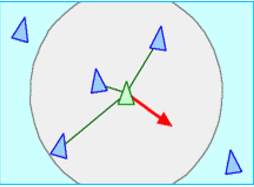
\includegraphics[width=0.35\textwidth]{imagenes/marco_teo/separation.png}
\caption{Separation behavior}
\label{img:separation-b}
\end{figure}

Por otro lado podemos encontrar el \textbf{alineamiento}~\ref{img:alignment-b} de la
dirección del movimento propio con las de las entidades más cercanas, de esta forma conseguimos un
movimiento armónico entre los \textit{boids} y produciremos una sensación de
coordinación entre ellos.

\begin{figure}[ht]
\centering
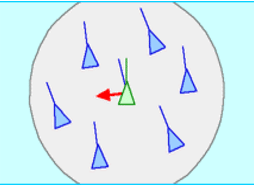
\includegraphics[width=0.35\textwidth]{imagenes/marco_teo/alignment.png}
\caption{Alignment behavior}
\label{img:alignment-b}
\end{figure}

Por último encontramos la \textbf{cohesión}~\ref{img:cohesion-b} la cual se encargará de
mantener a las entidades cercanas juntas para crear esa sensación de grupo que buscamos
con el algoritmo.

\begin{figure}[ht]
\centering
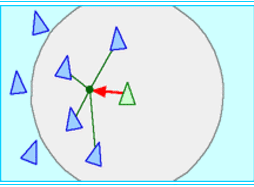
\includegraphics[width=0.35\textwidth]{imagenes/marco_teo/cohesion.png}
\caption{Cohesion behavior}
\label{img:cohesion-b}
\end{figure}

Por otro lado, podemos ver en el articulo de `Raynolds' como a lo largo de los años se
ha ido modificando y ampliando el algoritmo con el fin de añadir variaciones en el
comportamiento y/o introducir más factores influyentes en la decisión de los 
\textit{Boids} como puede ser el olor de determinada entidad/es y/o escenario. \\
Esto sin duda es gracias a la versatílidad que nos proporciona el uso de los
\textit{`Steering behaviors'} y jugar con la importancia de las distintas componentes
a la hora de hacer la toma de decisiones.

